\begin{frame}
    \frametitle{Imagen}
    
    \note{Ver libro de Sigwart. Seccion 4.2.3.2}
    \note{material sacado de mi tesis}
    \note{https://3d.bk.tudelft.nl/courses/geo1016/slides/Lecture_03_Calibration.pdf}
    
    \begin{columns}
    	\begin{column}{0.5\textwidth}
		    \begin{figure}[!h]
			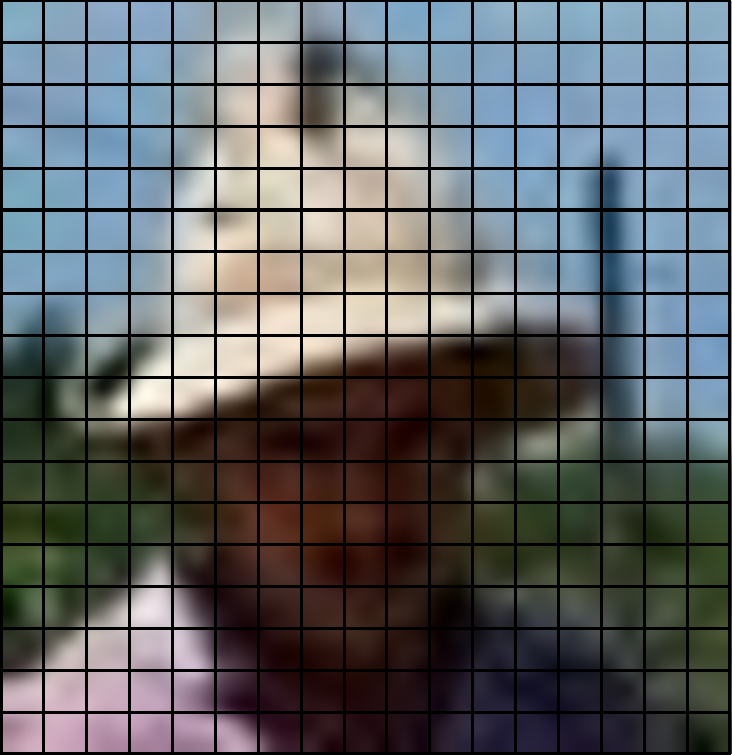
\includegraphics[width=0.6\columnwidth]{images/image_pixels.pdf}
			\end{figure}
    	\end{column}
    	\begin{column}{0.3\textwidth}
		Imagen color tiene 3 canales: R, G y B.
		\begin{equation*}
			f(x,y)=
			\begin{bmatrix}
				r(x,y) \\
				g(x,y) \\
				b(x,y)
			\end{bmatrix}
		\end{equation*}
    	\end{column}
    \end{columns}
\end{frame}

\begin{frame}
	\frametitle{Modelo de cámara Pinhole}
	
	\begin{figure}[!h]
		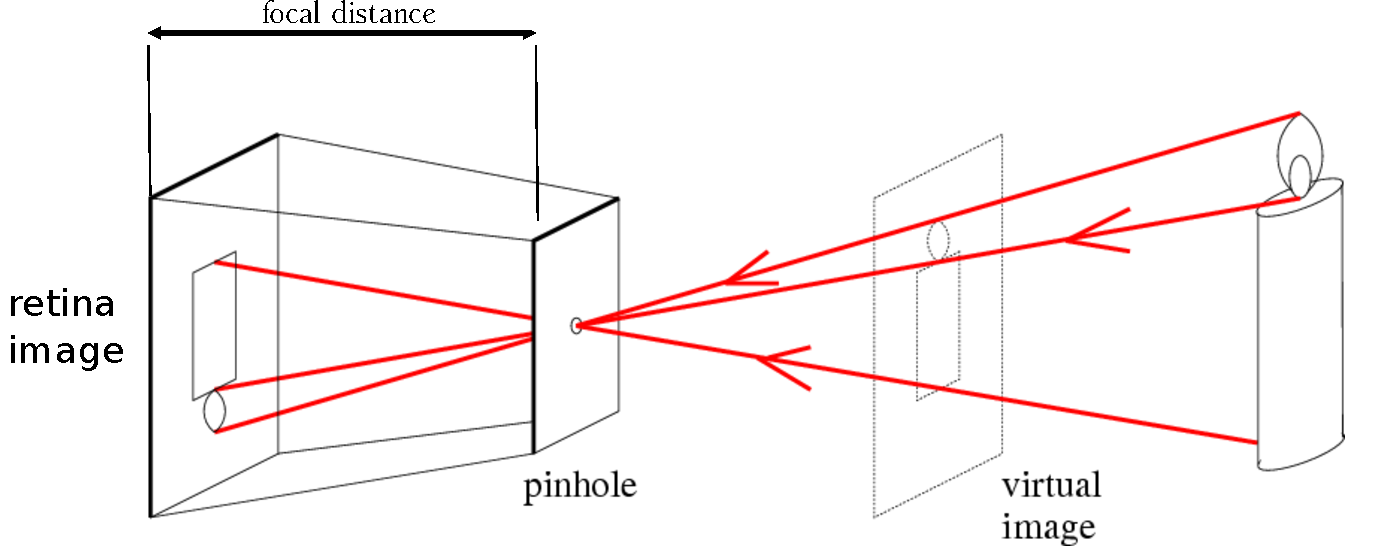
\includegraphics[width=0.6\columnwidth]{images/pinhole_camera_virtual_image.pdf}
	\end{figure}

\end{frame}

\begin{frame}
    \frametitle{Cámara - Modelo Pin-Hole}
    
    \note{Ver libro de Sigwart. Seccion 4.2.3.2}
    \note{material sacado de mi tesis}
    
    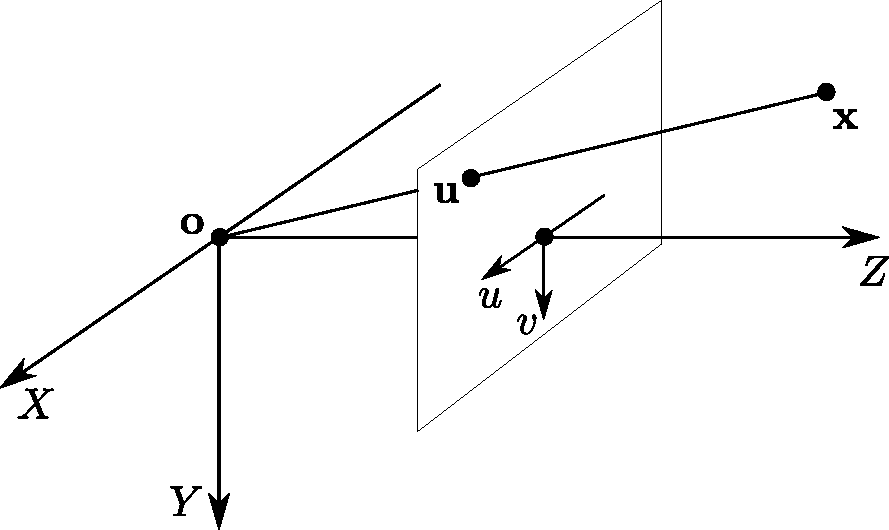
\includegraphics[width=0.4\columnwidth]{images/pinhole_camera_model.pdf}
    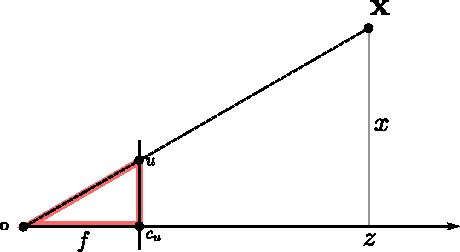
\includegraphics[width=0.4\columnwidth]{images/pinhole_camera_model2.pdf}
    \footnotesize
    
    \begin{block}{Principio de funcionamiento}
        En el modelo de cámara pinhole, el punto de la imagen $\imagePoint=\begin{bmatrix}u & v\end{bmatrix}^{\top}$ se determina como la intersección entre el plano de la imagen y el rayo que une el punto del mundo $\point =\begin{bmatrix}x & y & z\end{bmatrix}^{\top}$ y el centro de proyección $\cameraCenter$.
    \end{block}
    
    Denotamos con $\homo{\point}=\begin{bmatrix}x & y & z & 1\end{bmatrix}^{\top}$ la representación homogénea de un punto $\point=\begin{bmatrix}x & y & z\end{bmatrix}^{\top}$. Ahora, definimos el modelo de cámara:
    \begin{equation*}
        \imagePoint=f\proj(\cameraPoint)+\principalPoint
    \end{equation*}
    
    donde $f$ es la distancia focal, $\principalPoint$ es el punto principal, $\cameraPoint$ es el punto en el sistema de coordenadas de la cámara y la función $\proj:\mathbb{R}^{n}\rightarrow\mathbb{R}^{n- 1}$ se puede usar para transformar puntos de coordenadas homogéneas a no homogéneas, y también se puede usar para proyectar puntos del espacio 3D al plano de imagen 2D.	
\end{frame}

\begin{frame}
    \frametitle{Cámara - Modelo Pin-Hole}
    
    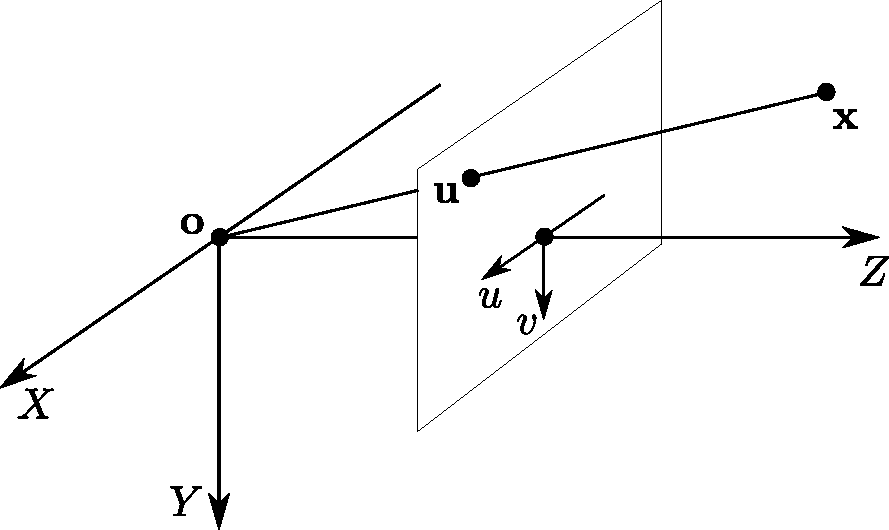
\includegraphics[width=0.4\columnwidth]{images/pinhole_camera_model.pdf}
    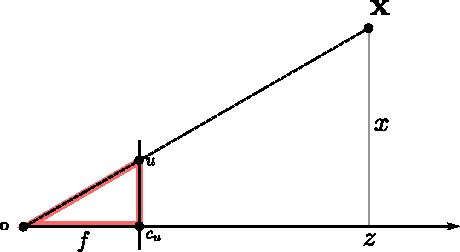
\includegraphics[width=0.4\columnwidth]{images/pinhole_camera_model2.pdf}
    \footnotesize
    
    \begin{equation*}
        \proj(\vec{a})=
        \frac{1}{a_{n}}\begin{bmatrix}a_{1}\\
            \vdots\\
            a_{n-1}
        \end{bmatrix}.
    \end{equation*}
    
    Por ejemplo, si $\point=\begin{bmatrix}x & y & z\end{bmatrix}^{\top}$, entonces $\proj(\point)=\begin{bmatrix}x/z & y/z\end{bmatrix}$.
    
    Se puede ver que $x/z=u/f$. Análogamente podemos decir que $y/z=v/f$. De estas ecuaciones podemos ver que $u=f(x/z)$ y que $v=f(y/z)$, por lo que la ecuación [eq:proyección] se cumple.
    
\end{frame}

%\begin{frame}
%    \frametitle{Cámara - Modelo Pin-Hole}
%    
%    \begin{figure}[!h]
%        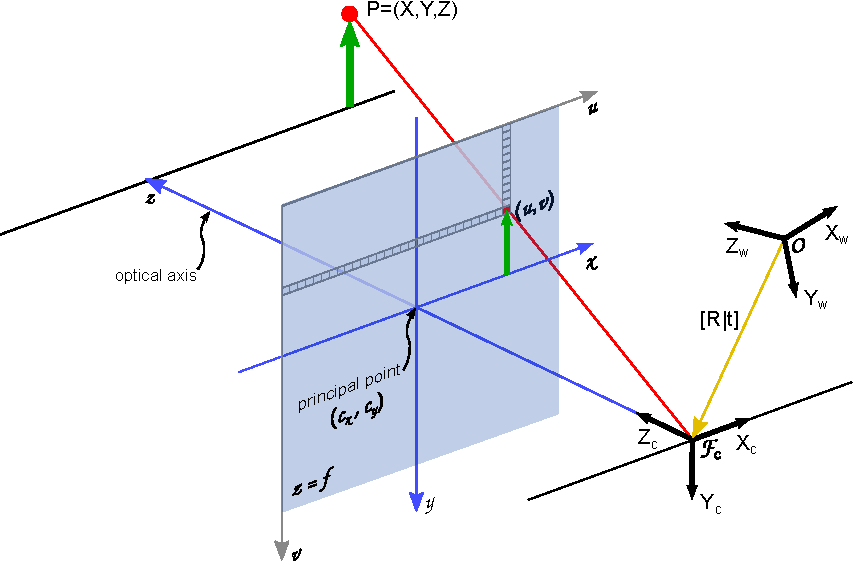
\includegraphics[width=0.6\columnwidth]{images/pinhole_camera_model3.pdf}
%    \end{figure}
%\end{frame}

